\documentclass{article}
\usepackage{tikz}
\usepackage{amsmath,amssymb}

\begin{document}

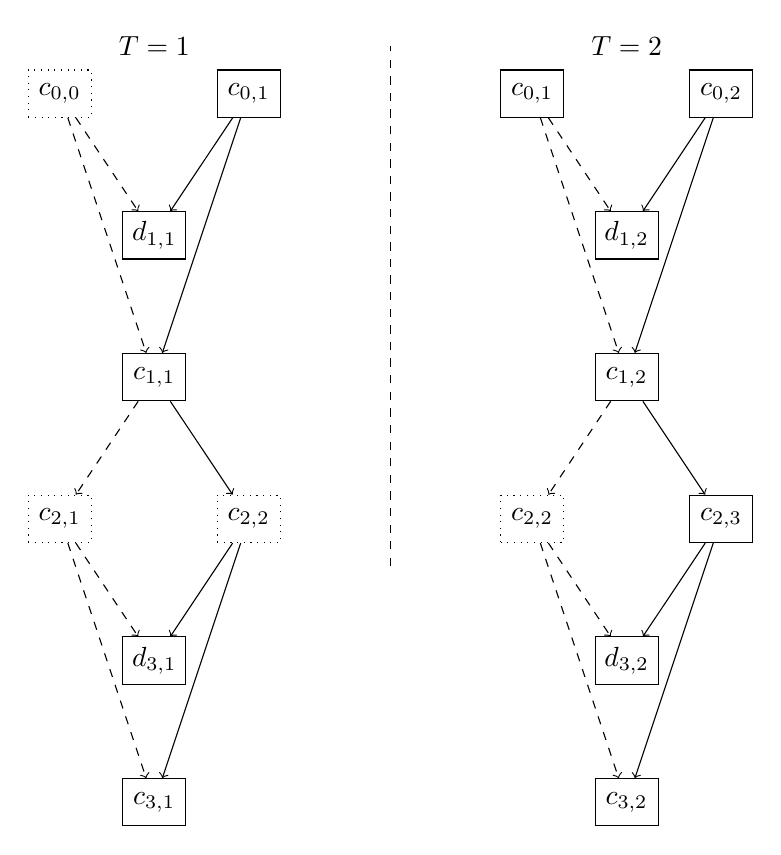
\begin{tikzpicture}[
    box/.style={draw, minimum width=0.8cm, minimum height=0.6cm},
    dotted box/.style={draw, dotted, minimum width=0.8cm, minimum height=0.6cm},
    scale=1.2
]

% Vertical dividing line
\draw[dashed] (4.5,-5) -- (4.5,0.5);

% T=1 label
\node at (2,0.5) {$T=1$};

% T=2 label
\node at (7,0.5) {$T=2$};

% T=1 side
% Top row
\node[dotted box] (t1c0) at (1,0) {$c_{0,0}$};
\node[box] (t1c1) at (3,0) {$c_{0,1}$};

% Second row
\node[box] (t1d1) at (2,-1.5) {$d_{1,1}$};
\draw[dashed, ->] (t1c0) -- (t1d1);
\draw[->] (t1c1) -- (t1d1);

% Third row
\node[box] (t1c2) at (2,-3) {$c_{1,1}$};
\draw[dashed, ->] (t1c0) -- (t1c2);
\draw[->] (t1c1) -- (t1c2);

% Fourth row
\node[dotted box] (t1c3) at (1,-4.5) {$c_{2,1}$};
\node[dotted box] (t1c4) at (3,-4.5) {$c_{2,2}$};
\draw[dashed, ->] (t1c2) -- (t1c3);
\draw[->] (t1c2) -- (t1c4);

% Bottom row
\node[box] (t1d3) at (2,-6) {$d_{3,1}$};
\draw[dashed, ->] (t1c3) -- (t1d3);
\draw[->] (t1c4) -- (t1d3);

% Final row
\node[box] (t1c6) at (2,-7.5) {$c_{3,1}$};
\draw[dashed, ->] (t1c3) -- (t1c6);
\draw[->] (t1c4) -- (t1c6);

% T=2 side
% Top row
\node[box] (t2c0) at (6,0) {$c_{0,1}$};
\node[box] (t2c1) at (8,0) {$c_{0,2}$};

% Second row
\node[box] (t2d1) at (7,-1.5) {$d_{1,2}$};
\draw[dashed, ->] (t2c0) -- (t2d1);
\draw[->] (t2c1) -- (t2d1);

% Third row
\node[box] (t2c2) at (7,-3) {$c_{1,2}$};
\draw[dashed, ->] (t2c0) -- (t2c2);
\draw[->] (t2c1) -- (t2c2);

% Fourth row
\node[dotted box] (t2c3) at (6,-4.5) {$c_{2,2}$};
\node[box] (t2c4) at (8,-4.5) {$c_{2,3}$};
\draw[dashed, ->] (t2c2) -- (t2c3);
\draw[->] (t2c2) -- (t2c4);

% Bottom row
\node[box] (t2d3) at (7,-6) {$d_{3,2}$};
\draw[dashed, ->] (t2c3) -- (t2d3);
\draw[->] (t2c4) -- (t2d3);

% Final row
\node[box] (t2c6) at (7,-7.5) {$c_{3,2}$};
\draw[dashed, ->] (t2c3) -- (t2c6);
\draw[->] (t2c4) -- (t2c6);

\end{tikzpicture}

\end{document}